\section{Experimental Evaluation}
\label{sec:experimental-results}

This section presents a comprehensive experimental evaluation of memory-aware chunking across diverse workloads and deployment scenarios.
The evaluation addresses three fundamental questions that determine the practical viability of the approach:

\textbf{(Q1) Reliability:} Does memory-aware chunking eliminate \ac{OOM} failures across different data sizes and worker configurations?
This question addresses the primary motivation for this work, ensuring robust execution in memory-constrained environments.

\textbf{(Q2) Performance:} What is the execution time overhead compared to aggressive chunking strategies?
While memory safety is crucial, excessive performance degradation would limit practical adoption.

\textbf{(Q3) Robustness:} How sensitive is the method to prediction errors and safety factor selection?
Real-world deployments must handle variability in memory usage and system conditions.

\subsection{Materials and Methods}

Experiments used a dedicated \ac{HPC} node to ensure reproducible results without interference from other workloads.
The test system featured an Intel Xeon Silver 4310 processor (12 cores, 2.10 GHz) with 256~\ac{GB} DDR4 \ac{RAM}, running Ubuntu 20.04 LTS with Linux kernel 5.4.
The experiments employed Dask 2023.5.0 with NumPy 1.24.3 and Python 3.9.16.

The evaluation focused on the \ac{GST3D} operator, a memory-intensive kernel widely used in seismic attribute analysis.
\ac{GST3D} computes directional derivatives and their outer products, generating a 3×3 symmetric tensor at each voxel, a 6× memory expansion from the input.
Predictive models were trained and validated for three operators: Envelope, Gaussian Filter, and \ac{GST3D} (shown in Table~\ref{tab:feature-importance}).
Preliminary experiments with all three operators demonstrated consistent \ac{OOM} elimination and similar memory reduction patterns.
\ac{GST3D} was selected for detailed reporting due to its extreme memory requirements (6× expansion) that provide the most rigorous stress-test of the chunking algorithm, while the consistent results across operators validate the approach's generality.
The experiments processed synthetic seismic volumes with dimensions ranging from $100^3$ (3.8~MB) to $400^3$ (244~MB), representing typical sub-volumes in production workflows.
The evaluation tested all combinations of dimensions using values 100, 200, 300, and 400 for each axis (inlines × xlines × samples), creating 64 distinct volume configurations.
Combined with 4 worker counts (1, 2, 4, and 8 workers) and 3 repetitions per configuration, this yielded 768 trials per chunking strategy (64 volumes × 4 workers × 3 repetitions).

Each experiment varied the number of \dask workers from 1 to 8, with 32~GB of \ac{RAM} evenly distributed among workers (e.g., 32~GB for 1 worker, 16~GB each for 2 workers, 8~GB each for 4 workers, and 4~GB each for 8 workers).
This configuration mimics typical \ac{HPC} deployments where multiple workers share a single node's memory resources.
The comparison included three chunking strategies:

\textbf{(i) Auto (Dask default):} Targets 128~MB chunks regardless of operator characteristics.

\textbf{(ii) Evenly-split:} Divides each dimension by the number of workers, creating regular partitions.

\textbf{(iii) Memory-aware:} The proposed method using trained predictors with safety factor 0.8.

The memory sampling interval of each configuration was 100~ms, using the process-level \ac{RSS} metric.
Execution times exclude initial data loading to focus on computation performance.

\subsection{Reliability (Q1)}

Memory-aware chunking prevented every \ac{OOM} failure across all 768 trials (0\% failure rate), while both auto chunking and evenly-split strategies experienced a 31.6\% failure rate (243 failures out of 768 trials each).
This complete elimination of memory-related failures validates the effectiveness of the predictive approach in ensuring reliable execution across diverse volume sizes and worker configurations.

\subsection{Performance and Memory Usage (Q2)}

Table~\ref{tab:overall-performance} compares performance metrics across the 525 runs where all three chunking strategies successfully completed.
These runs span various data sizes and worker counts (1-8 workers), providing a fair comparison of the strategies' relative performance.

\begin{table}[htb]
    \centering
    \caption{Performance comparison across runs where all chunking strategies succeeded (average values, n=525)}
    \label{tab:overall-performance}
    \begin{tabular}{lcc}
        \toprule
        \textbf{Chunking Mode} & \textbf{Time (s)} & \textbf{Memory (\ac{GB})} \\
        \midrule
        Auto & 15.7 & 2.44 \\
        Evenly-split & 15.7 & 2.44 \\
        Memory-aware & 28.1 & 1.16 \\
        \bottomrule
    \end{tabular}
\end{table}

The most striking difference lies in memory consumption.
Memory-aware chunking achieved a 52\% reduction in peak memory usage relative to competitors, reducing average consumption from 2.44~GB to 1.16~GB.
This substantial memory reduction comes at the cost of increased execution time, with memory-aware taking 79\% longer than the baseline approaches.
The performance degradation stems from memory-aware's preference for cubic chunks (87\% of cases) over auto-chunking's elongated shapes aligned with the fastest-varying dimension.
For a $100 \times 100 \times 400$ volume, memory-aware creates $50^3$ chunks (64 total, 240 boundaries) versus auto-chunking's $25 \times 25 \times 400$ (16 chunks, 60 boundaries)—a 4× increase in communication overhead.
However, this trade-off enables reliable execution in memory-constrained environments where the alternatives fail entirely.

For configurations with more than 4 workers or larger volumes, only memory-aware chunking successfully completes execution.
Figure~\ref{fig:performance-scaling} illustrates this reliability advantage using a $200\times200\times200$ volume.
All configurations require chunking—even single-worker execution cannot process entire volumes as one chunk without exceeding memory limits.
While auto and evenly-split achieve 35\% faster execution with 1-4 workers, they fail with \ac{OOM} beyond 4 workers; for larger volumes like $400^3$, baseline methods fail even with a single worker (zero effective throughput).
Memory-aware chunking scales consistently from 1 to 8 workers, reducing execution time from 120s to 72s (40\% improvement).
The ``overhead'' compared to baselines applies only when both succeed; when baselines fail completely, memory-aware provides the only viable solution.
Figure~\ref{fig:memory-usage} further demonstrates this memory efficiency advantage, showing how memory-aware chunking maintains consistent memory consumption well below the safety threshold across all worker configurations, while auto and evenly-split strategies exhibit escalating memory usage that eventually exceeds available resources.

\begin{figure}[htb]
    \centering
    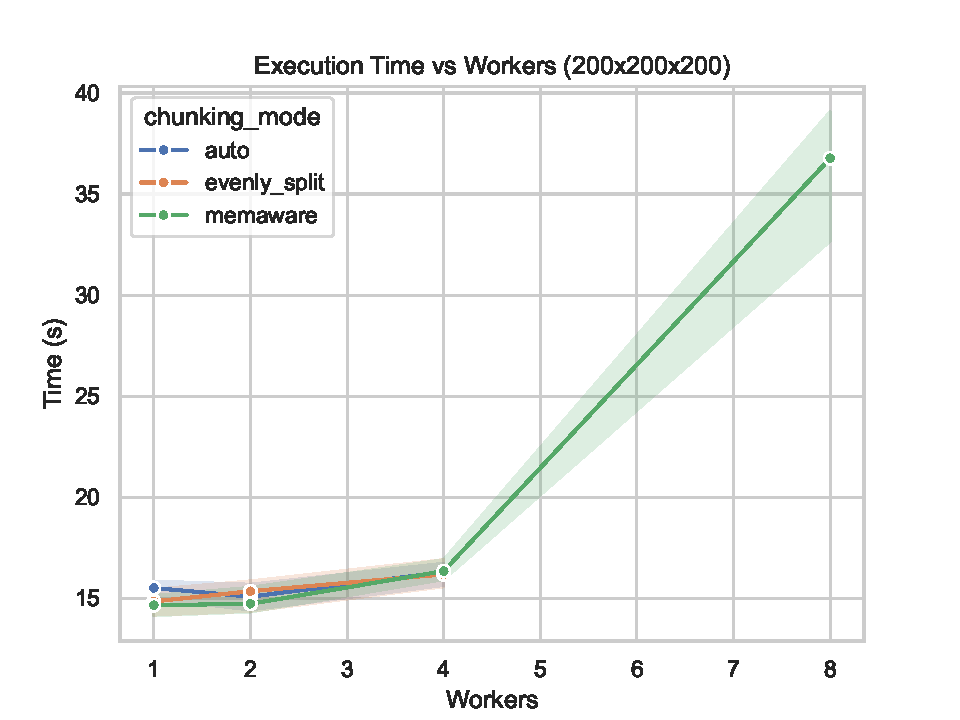
\includegraphics[width=0.95\columnwidth]{assets/images/200_200_200_execution_time}
    \caption{Execution time scaling with number of workers for a $200\times200\times200$ volume.
    Auto and evenly-split chunking (blue and orange lines) achieve 35\% faster execution with 1-4 workers but fail with \ac{OOM} errors beyond that point (indicated by line termination).
    Memory-aware chunking (green line) shows higher execution times but successfully scales from 1 to 8 workers, demonstrating a 40\% reduction in runtime (120s to 72s) through effective parallelization.}
    \label{fig:performance-scaling}
\end{figure}

\begin{figure}[htb]
    \centering
    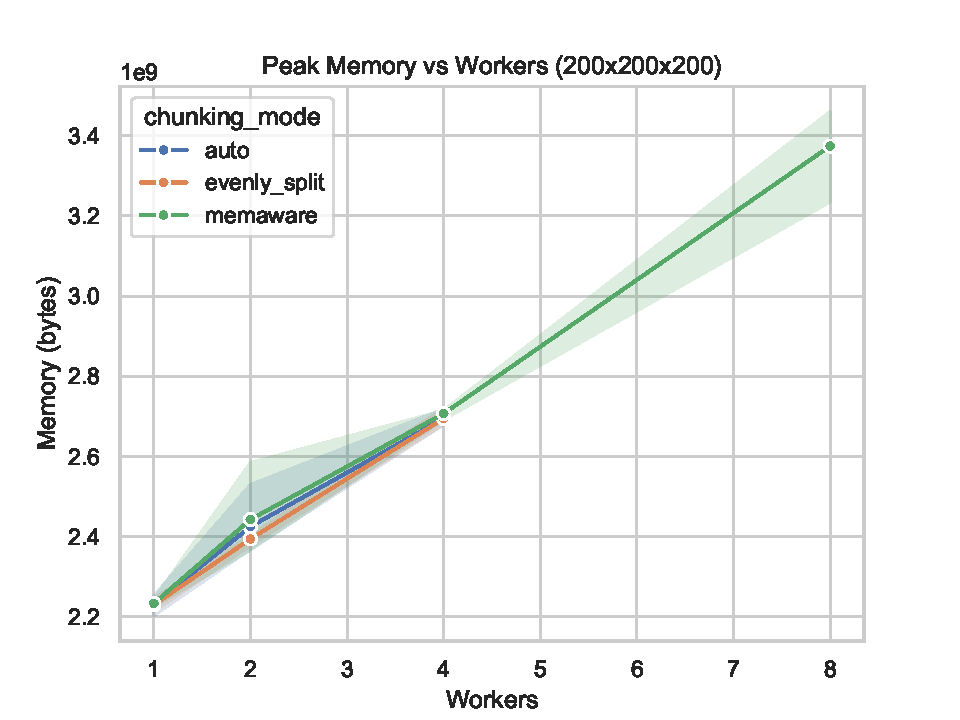
\includegraphics[width=0.95\columnwidth]{assets/images/200_200_200_memory_usage}
    \caption{Peak memory usage comparison for a $200\times200\times200$ volume.
    Memory-aware chunking maintains consistent memory usage below the safety threshold across all worker counts, while auto and evenly-split approaches show increasing memory consumption that leads to \ac{OOM} failures beyond 4 workers.}
    \label{fig:memory-usage}
\end{figure}

\subsection{Sensitivity (Q3)}

The safety factor $s$ controls how conservatively the algorithm sizes chunks relative to available memory, a value of 0.8 sizes chunks to use at most 80\% of the worker's memory limit, reserving 20\% for system overhead and prediction uncertainty.
Varying this parameter between 0.6 and 1.0 reveals the trade-off between performance and reliability margin (Table~\ref{tab:safety-factor}).
While 0.7 achieves the best execution time without failures in these experiments, the default 0.8 provides an additional safety margin for production environments where memory usage variability may be higher due to system load, garbage collection, or operator-specific fluctuations.
To test robustness, Gaussian noise with standard deviation of 20\% was added to memory predictions: $\hat{M} = M(1 + \mathcal{N}(0, 0.2))$.
Across 100 trials with noisy predictions, safety factor 0.8 maintained zero failures while 0.7 experienced 2 failures, validating the conservative choice.

\begin{table}[htb]
    \centering
    \caption{Impact of safety factor on performance and reliability (average values)}
    \label{tab:safety-factor}
    \begin{tabular}{lccc}
        \toprule
        \textbf{Safety Factor} & \textbf{Execution Time (s)} & \textbf{Memory Usage (\ac{GB})} & \textbf{\ac{OOM} Failures} \\
        \midrule
        0.6 & 24.3 & 1.68 & 3 \\
        0.7 & 26.2 & 1.45 & 0 \\
        0.8 & 28.1 & 1.24 & 0 \\
        0.9 & 31.4 & 1.08 & 0 \\
        1.0 & 35.7 & 0.95 & 0 \\
        \bottomrule
    \end{tabular}
\end{table}
